
\makequotation{It is practically impossible to teach good programming to
  students that have had a prior exposure to BASIC: as potential
  programmers they are mentally mutilated beyond hope of
  regeneration.}{Edsger W. Dijkstra, Turing Award winner}

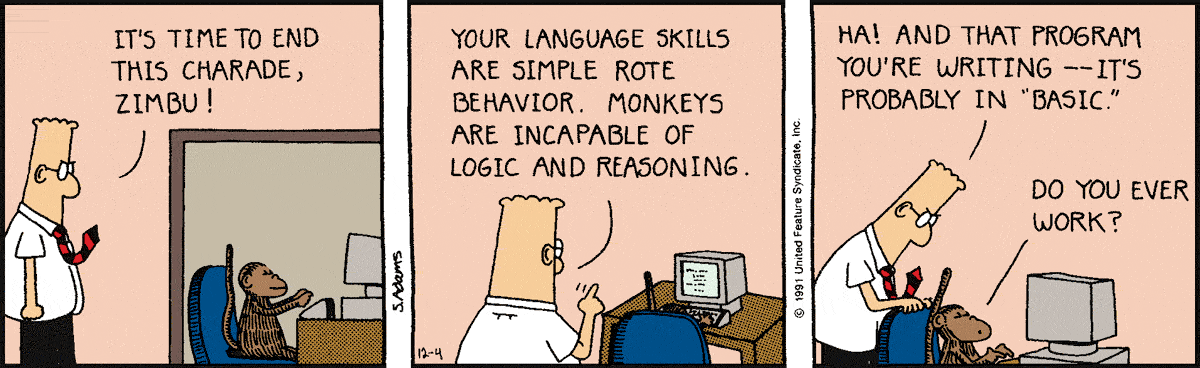
\includegraphics[width=\textwidth]{figs/dilbert-1991-12-04.png}

%% \makequotation{\ldots the teaching of BASIC should be rated as a
%%   criminal offence: it mutilates the mind beyond recovery.}{Edsger
%%   W. Dijkstra, Turing Award winner}

%% \makequotation{I think it's fair to say that more persons in the world know how to
%% write simple programs in BASIC than in any other language. It is true
%% that most of them are probably still unable to vote or buy a drink.  And
%% if FORTRAN is the lingua franca, then certainly it must be true that
%% BASIC is the lingua playpen.}{Thomas E. Kurtz, co-creator of BASIC, in
%%   1981~\cite{hopl}} 

Much has been written over the decades about the democratization of
computers thanks to Moore's Law, but what has been overlooked is that up
until the consumer Internet appeared in around 1995, BASIC was present
at every milestone, and played a pivotal role in empowering generations
of programmers.
Yet BASIC is probably one of the most maligned programming languages
to achieve widespread use.

In \emph{Back to BASIC}~\cite{backtobasic}, the language's co-creators
object that the criticisms leveled at the 
BASIC dialects that proliferated after BASIC became the
\emph{lingua franca} of PCs did not apply to the original language
they had created and to its designated descendants.
This defense seems doubtful, since the original language did include
\T{GO~TO}, which Dijkstra famously railed
against~\cite{goto_considered_harmful}.

Nonetheless, even if we grant the criticisms,
they miss the goal of the
language, which was to expose as many non-programmers as possible to
programming---something it accomplished beyond its creators' wildest dreams,
if not in the precise way they had envisioned.
BASIC introduced an entire generation of
programmers to programming.  If it inculcated ``bad'' habits that
structured languages tried to break,  it also taught us computational
thinking.    It's time the true story of BASIC's influence was told.

%% TBD need to give due credit to Gates, Allison and PC makers here
